\lesson{9}{8.11.2023}{Сортировки. Сжатие и защита информации.}

\section{Сортировка Хоара (быстрая сортировка)}
Идея: выберем элемент-разделитель. Разместим все меньшие разделителя элементы
слева от него, большие — справа и запустим процесс для каждой из частей.
\begin{eg}
    
    $\newline$
    \begin{verbatim}
        38 27 43 3 9 82 10 (pivot is 3)
        3 27 38 43 9 82 10 (pivot is 38)
        3 27 10 9 38 43 82 (pivot is 27)
        3 10 9 27 38 43 82 (pivot is 10)
        3 9 10 27 38 43 82 (pivot is 9)
        3 9 10 27 38 43 82
    \end{verbatim}
\end{eg}

\section{Пирамидальная сортировка (иерархическая, heapsort)}
\begin{enumerate}
    \item \textbf{Построение кучи:} Преобразуем исходный массив в максимальную кучу. В максимальной куче значение каждого узла больше или равно значению его потомков.
    \item \textbf{Сортировка:} Удаляем максимальный элемент (корень кучи), заменяем его последним элементом кучи, уменьшаем размер кучи на один и восстанавливаем свойство кучи. Повторяем, пока в куче не останется элементов.
\end{enumerate}

\begin{eg}
    Построение кучи (массив $a = [38, 27, 43, 3, 9, 82, 10]$):

    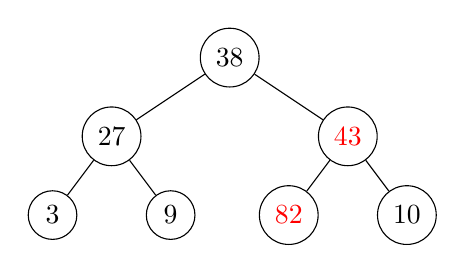
\begin{tikzpicture}[level distance=1cm,
        level 1/.style={sibling distance=3cm},
        level 2/.style={sibling distance=1.5cm}]
        \node[circle,draw] {38}
          child {node[circle,draw] {27}
            child {node[circle,draw] {3}}
            child {node[circle,draw] {9}}
          }
          child {node[circle,draw, text=red] {43}
          child {node[circle,draw, text=red] {82}}
          child {node[circle,draw] {10}}
          };
      \end{tikzpicture}

      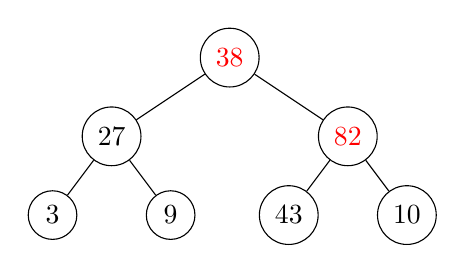
\begin{tikzpicture}[level distance=1cm,
        level 1/.style={sibling distance=3cm},
        level 2/.style={sibling distance=1.5cm}]
        \node[circle,draw,text=red] {38}
          child {node[circle,draw] {27}
            child {node[circle,draw] {3}}
            child {node[circle,draw] {9}}
          }
          child {node[circle,draw,text=red] {82}
          child {node[circle,draw] {43}}
          child {node[circle,draw] {10}}
          };
      \end{tikzpicture}

      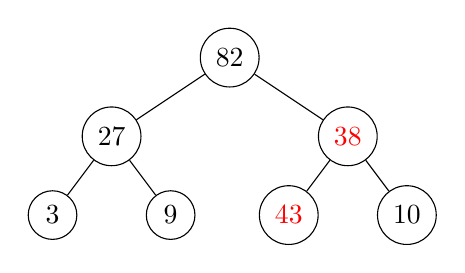
\begin{tikzpicture}[level distance=1cm,
        level 1/.style={sibling distance=3cm},
        level 2/.style={sibling distance=1.5cm}]
        \node[circle,draw] {82}
          child {node[circle,draw] {27}
            child {node[circle,draw] {3}}
            child {node[circle,draw] {9}}
          }
          child {node[circle,draw, text=red] {38}
          child {node[circle,draw, text=red] {43}}
          child {node[circle,draw] {10}}
          };
      \end{tikzpicture}
      
      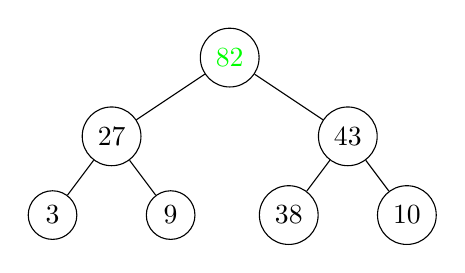
\begin{tikzpicture}[level distance=1cm,
        level 1/.style={sibling distance=3cm},
        level 2/.style={sibling distance=1.5cm}]
        \node[circle,draw,text=green] {82}
          child {node[circle,draw] {27}
            child {node[circle,draw] {3}}
            child {node[circle,draw] {9}}
          }
          child {node[circle,draw] {43}
          child {node[circle,draw] {38}}
          child {node[circle,draw] {10}}
          };
      \end{tikzpicture}
    
    Далее меняем местами 82 и 10, удаляем 82 из кучи и восстанавливаем свойство кучи.
\end{eg}

\section{Порозрядная сортировка (radix sort)}

Если известно, что диапазон ключей ограничен, то сортировать можно значительно
быстрее: сортируем последовательно по разрядам (например, по десятичным или
двоичным), начиная с младшего. (Пример придумайте сами)


\chapter{Сжатие и защита информации}

\section{Задача о префиксном коде.}


Пусть $A = \{c_1, \ldots, c_n\}$ --- алфавит, $p_1, \ldots, p_n$ --- вероятности появления символов. Пусть задан код $\phi: A \to \{0, 1\}^*$\\
Фиксируем текст (большую строку) длины $N: a_1 a_2\ldots a_N$. В этом тексте количество символов $c_i$ -- $N \cdot a_i$ (закон больших чисел). Тогда длина кодовой последовательности текста:

\[\sum_{i=1}^{n} N p_i \phi(c_i)\]
Задача заключается в том, чтобы минимализировать длину кодовой последовательности такого текста,
а т.к. $N$ -- фиксированная величина, не влияющая на коды, задача сводиться к тому, чтобы минимализировать сумму:
\[\sum_{i=1}^{n}p_i \phi(c_i)\]
При этом для $p_i, \phi(c_i)$ выполняются:
\begin{enumerate}
    \item $\sum p_i = 1$
    \item $0 < p_i < 1$
    \item $\phi(c_i) \in \N$
    \item $\phi(c_1), \ldots, \phi(c_n)$ -- длины кодов символов в префиксом коде, т.е. для этих длин выполняется неравенство Крафта.
\end{enumerate}

Алгоритм решения такой задачи основывается на нескольких свойств длин кодовых последовательностей:
\begin{lemma}
    Пусть $p_i$ -- вероятности символов и $s_i$ -- длины кодов символов для оптимального кода.

    Если $p_1 \geqslant p_2 \geqslant...\geqslant p_m$, то $s_1 \leqslant s_2 \leqslant...\leqslant s_m$.
\end{lemma}

\begin{proof}
    Мы просто покажем, что если найдутся две пары чисел $(p_i, s_i)$ и $(p_j,s_j)$, такие что $p_i < p_j$ и $s_i < s_j$, то значение суммы попарных произведений можно уменьшить, заменив эти две пары парами $(p_i, s_j)$ и $(p_j, s_i)$. Действительно, т.к. $(p_j - p_i)(s_j - s_i) > 0$, то, раскрывая скобки, получим после элементарных преобразований $p_is_i+p_js_j>p_is_j+p_js_i$.

    Так как число возможных расположений конечно, поскольку равно $m!$, то начиная с любого расположения за конечное число шагов мы закончим процесс улучшений на расположении, которое дальше улучшить невозможно. На нём и достигается минимум.
\end{proof}

\begin{lemma}
    Две самые длинные кодовые последовательности имеют одинаковую длину.
\end{lemma}

\begin{proof}
    Предположим, что $s_{m-1} < s_m$. Тогда в силу префиксности кода, можно отбросить лишние символы из кода $s_m.$ Мы получим снова префиксный код, но с меньшим значением целевой функции. Противоречие.
\end{proof}

\begin{lemma}
    Рассмотрим задачу $P'$, которая получается объединением двух самых редких символов в один символ. Минимальное значение целевой функции 
    в задаче $P'$ будет отличаться от значения в задаче $P$ на $p'_{m-1} = p_{m-1} +p_m$, а оптимальный кодовый
    набор для $P$ получается из решения задачи $P'$ удлинением на 1 бит кодовых последовательностей для символов, которые были объединены.
\end{lemma}

\begin{proof}
    Пересчитываем новую функцию:

$\sigma(P)=\sum\limits_{i=1}^{m-2}p_is_i+(s'_{m-1}+1)p_{m-1}+(s'_{m-1}+1)p_m=$

$=\sum\limits_{i=1}^{m-2}p_is_i+s'_{m-1}(p_{m-1}+p_m)+p_{m-1}+p_m=\sigma_{опт}(P')+p'_{m-1}$.

Осталось доказать, что построенный код для $P$ действительно оптимальный.

Предположим, что существует решение для $P$, такое что $\sigma^*(P)<\sigma(P).$ По лемме 2 длины кодов самых редких символов равны. Объединим эти символы в один, а код для него построим откидыванием последнего бита. В силу префиксности кода для $P$ это можно сделать.

Таким образом, получили префиксный код для задачи $P'$, и при этом $\sigma^*(P') < \sigma(P').$ Противоречие.
\end{proof}

\section{Код Шеннона-Фано и алгоритм Хаффмана}


Кодирование Шеннона — Фано — алгоритм префиксного неоднородного кодирования. Относится к вероятностным методам (т.е. мера на множестве событий, принимающая значения от $0$ до $1$) сжатия. 


Часто встречающийся символ кодируется кодом меньшей длины (короткой двоичной последовательностью), редко встречающийся — кодом большей длины (длинной двоичной последовательностью).

\begin{algoritm}[Хаффмана]
    Лемма 3 фактически даёт нам алгоритм для построения оптимального кода:
    \begin{enumerate}
        \item Составим список кодируемых символов вместе с их частотами. Каждый символ представим в виде одноэлементного дерева с соответствующим весом.
        \item Из списка выберем два дерева с наименьшими весами.
        \item Создадим новый корень и назначим ему в качестве детей эти два дерева. Вес сформированного дерева положим равным сумме весов дочерних. Таким образом, два дерева “склеились” в одно.
        \item Добавим новое дерево в список.
        \item Если в списке осталось ровно одно дерево, закончить процесс, иначе - перейти к п.2.
    \end{enumerate}
\end{algoritm}

\begin{eg}
    Пусть $A = \{a, b, c, d, e\}$, $p_a = 0.37, p_b = 0.22, p_c = 0.16, p_d = 0.14, p_e = 0.11$.
    
    Объединим $d$ и $e$ в один символ $de$ с вероятностью $0.25$. Тогда получим следующее дерево:
    
    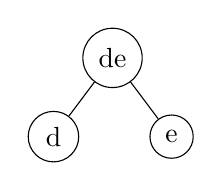
\begin{tikzpicture}[level distance=1cm,
        level 1/.style={sibling distance=1.5cm},
        level 2/.style={sibling distance=1.5cm}]
        \node[circle,draw] {de}
          child {node[circle,draw] {d}}
          child {node[circle,draw] {e}};
    \end{tikzpicture}
    
    На следующем шаге объединим $c$ и $b$ в один символ $bc$ с вероятностью $0.38$. Тогда получим следующее дерево:

    \begin{minipage}{.5\textwidth}
        \centering
        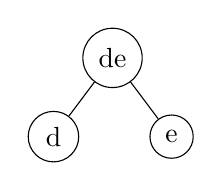
\begin{tikzpicture}[level distance=1cm,
            level 1/.style={sibling distance=1.5cm},
            level 2/.style={sibling distance=1.5cm}]
            \node[circle,draw] {de}
              child {node[circle,draw] {d}}
              child {node[circle,draw] {e}};
        \end{tikzpicture}

    \end{minipage}%
    \begin{minipage}{.5\textwidth}
        \centering
        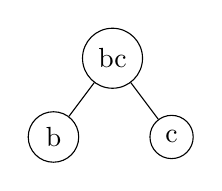
\begin{tikzpicture}[level distance=1cm,
            level 1/.style={sibling distance=1.5cm},
            level 2/.style={sibling distance=1.5cm}]
            \node[circle,draw] {bc}
              child {node[circle,draw] {b}}
              child {node[circle,draw] {c}};
        \end{tikzpicture}

    \end{minipage}

    Следующий шаг:
    
    \begin{minipage}{.5\textwidth}
        \centering
        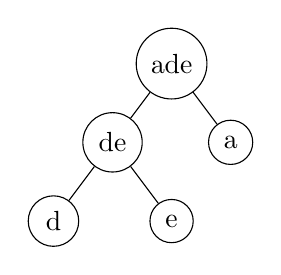
\begin{tikzpicture}[level distance=1cm,
            level 1/.style={sibling distance=1.5cm},
            level 2/.style={sibling distance=1.5cm},
            level 3/.style={sibling distance=1.5cm}]
            \node[circle,draw] {ade}
              child {node[circle,draw] {de}
                child {node[circle,draw] {d}}
                child {node[circle,draw] {e}}} 
              child {node[circle,draw] {a}};
        \end{tikzpicture}

    \end{minipage}%
    \begin{minipage}{.5\textwidth}
        \centering
        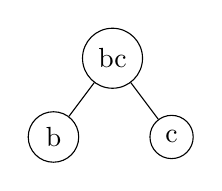
\begin{tikzpicture}[level distance=1cm,
            level 1/.style={sibling distance=1.5cm},
            level 2/.style={sibling distance=1.5cm}]
            \node[circle,draw] {bc}
              child {node[circle,draw] {b}}
              child {node[circle,draw] {c}};
        \end{tikzpicture}

    \end{minipage}

    Последний шаг:

    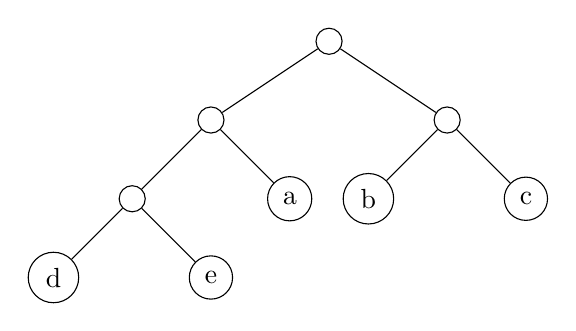
\begin{tikzpicture}[level distance=1cm,
        level 1/.style={sibling distance=3cm},
        level 2/.style={sibling distance=2cm}, % Increase this value
        level 3/.style={sibling distance=2cm}]
        \node[circle,draw] {}
          child {node[circle,draw] {}
            child {node[circle,draw] {}
              child {node[circle,draw] {d}}
              child {node[circle,draw] {e}}} 
            child {node[circle,draw] {a}}}
          child {node[circle,draw] {}
            child {node[circle,draw] {b}}
            child {node[circle,draw] {c}}};
    \end{tikzpicture}

    Коды для символов: $a = 01, b = 10, c = 11, d = 000, e = 001$.
\end{eg}